\chapter{Background}
\label{ch:background}

% Describe protocols and systems your work depends on.
% In almost all cases, this should contain a section on SCION.

% Started in 2009 (15y ago)
% The SCION Internet became operational in 2017

In this chapter we give some background information needed to understand the following chapters.


\section{SCION}

SCION \cite{Perrig2022} is a clean-slate Internet architecture focused on scalability, control and isolation and is designed to provide security, flexibility, and performance improvements over the current Internet.
In this section we will go over the main concepts of SCION, explain some details about ...


\subsection{Core Concepts}
In the following we explain SCION's core features and how it achieves them.
\subsubsection{Isolation}

By putting the different autonomous systems (ASes) into groups called isolation domains (ISD), as seen in \cref{fig:scion_isd_architecture}, SCION can provide isolation between them.
Every ISD has some core ASes which administer the ISD, form the root of trust of the ISD and provide connectivity to other ISDs.
The configuration of an ISD is stored in a signed file called trust root configuration (TRC), which includes for example root certificates or policies.
If there happens a misconfiguration in an ISD, only this ISD is affected and the rest of the Internet can still operate.

\begin{figure}
    \centering
    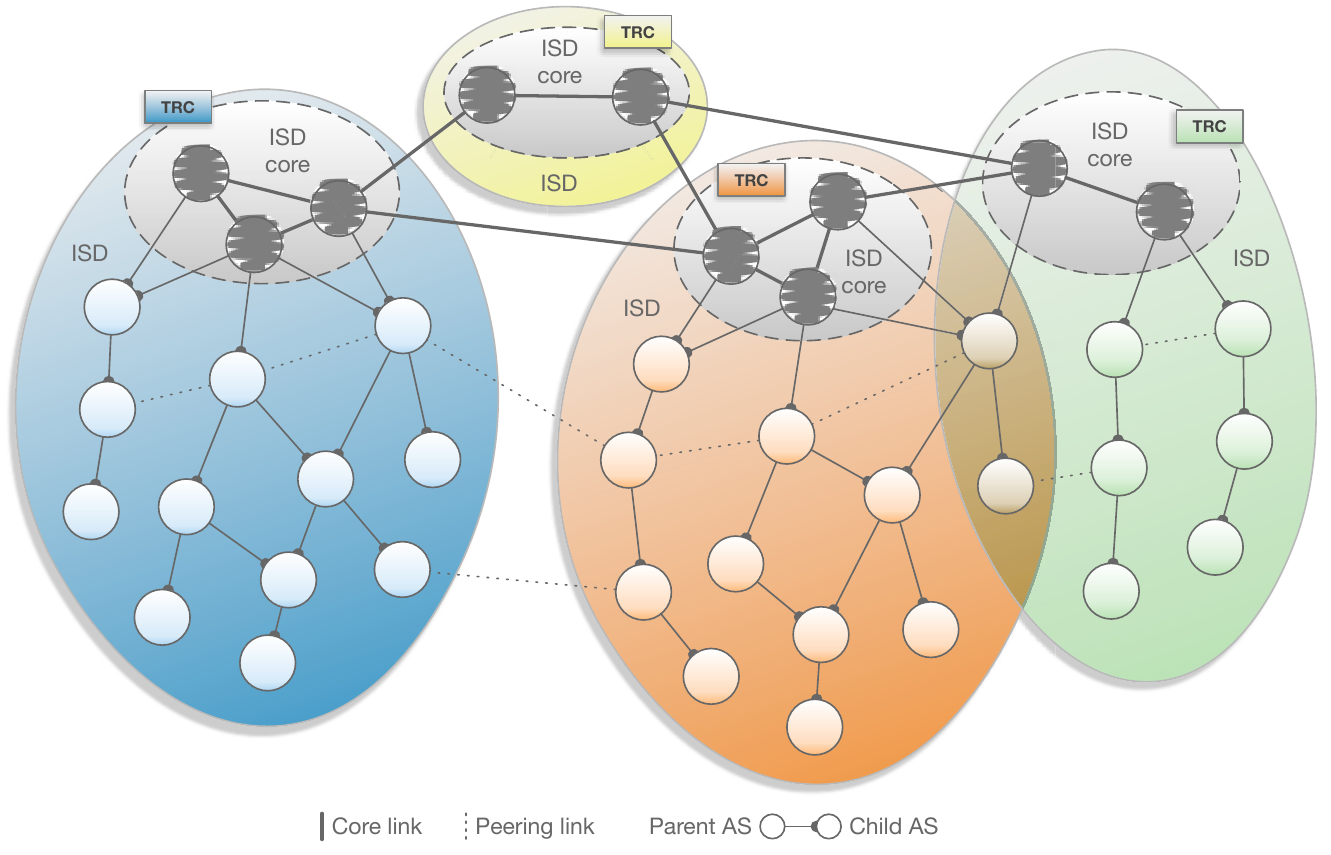
\includegraphics[width=0.75\textwidth]{figures/scion_isd_architecture.png}
    \caption{SCION Architecture with ISD and ASes. ASes are represented by circles. Figure taken form Chapter 2 of the SCION book \cite{Perrig2022}.}
    \label{fig:scion_isd_architecture}
\end{figure}


\subsubsection{Control}

SCION offers users the ability to request and select the best paths for their network traffic to the desired destinations.
This allows omitting certain regions or countries that the user does not trust and that may perform some sort traffic analysis.
The user is not limited to just use a single path.
With the option to utilize multiple paths simultaneously, SCION empowers users with greater control and flexibility over their network traffic.
This multipath feature ensures also higher availability in case of a network issue along a path.


\subsubsection{Scalability}

The path information in SCION packets is stored in the SCION packet header.
Based on this information, the SCION routers can forward the packets to the next hop and thus do not to store any state information and do not need to perform the expensive longest prefix matching.
The concept of ISD has also an impact on the scalability of SCION.
It allows splitting up the routing processes into two levels:
One for routing within an ISD and one for routing between ISDs.


\subsection{Path Construction}

\subsubsection{Control Plane}
PCB
MAC calculation for hop
\subsubsection{Data Plane}
Segment combination
header (info + hopfield)



SPAO + DRKey

\section{Anapaya}



\section{Security Tools}


\subsection{Automatic Scanning Tools}
We mainly use Nessus and OpenVAS to scan and automatically detect potential vulnerabilities on the SCION devices.
The primary difference between Nessus and OpenVAS is that Nessus is a proprietary tool, while OpenVAS is open-source.
Both tools are free to use and can run unauthenticated as well as authenticated scans.
Since the authenticated scans use credentials to log in to the target device, they can gather more information about the device and provide more accurate results.
At the end of a scan, both tools generate reports that give a detailed overview of the vulnerabilities and weaknesses found on the scanned devices.




